% Figures/subgradient.tex
% Illustrates Definition \ref{def:subgradient} and Theorem
% \ref{thm:subgradient-exists} of Chapter \ref{ch:convex}: at a kink of a convex
% function the subdifferential is the whole interval of slopes of supporting
% affine functions. The function drawn is f(x) = max{1.5 - x, 2x - 1.5}, with
% the kink at x_0 = 1 and f(x_0) = 0.5. The extreme supporting slopes -1 and 2
% are the one-sided derivatives; the slope 1/2 line is one interior element of
% the subdifferential.
\begin{tikzpicture}[
		scale=1.35,
		>=stealth,
		curve/.style={line width=1.3pt},
		support/.style={line width=0.7pt, black!60},
		guide/.style={line width=0.4pt, black!35, dashed},
	]

	\draw[->,line width=0.5pt] (-0.15,0) -- (2.95,0) node[right,font=\small] {$x$};
	\draw[->,line width=0.5pt] (0,-0.9) -- (0,2.35);

	% supporting affine functions through (1, 0.5)
	% slope -1 : y = 1.5 - x
	\draw[support] (1,0.5) -- (2.60,-1.10);
	% slope 1/2 : y = 0.5x
	\draw[support] (0.10,0.05) -- (2.80,1.40);
	% slope 2   : y = 2x - 1.5
	\draw[support] (0.35,-0.80) -- (1,0.5);

	% the function itself
	\draw[curve] (0.10,1.40) -- (1,0.5) -- (1.85,2.20);

	\draw[guide] (1,0) -- (1,0.5);
	\fill (1,0.5) circle (1.7pt);
	\node[font=\scriptsize,anchor=north] at (1,-0.06) {$x_0$};

	\node[font=\small,anchor=south west] at (1.83,2.16) {$f$};
	\node[font=\scriptsize,anchor=north west,black!60] at (2.58,-1.06)
	{slope $-1$};
	\node[font=\scriptsize,anchor=west,black!60] at (2.82,1.40)
	{slope $\tfrac12$};
	\node[font=\scriptsize,anchor=north east,black!60] at (0.42,-0.78)
	{slope $2$};

\end{tikzpicture}
